Chao et al. \cite{chaoLFSRDiffLightField2025} propose a U-Net architecture for processing light field data.
The architecture makes use of the disentanglement mechanism introduced by Wang et al. \cite{wangDisentanglingLightFields2023}.

\begin{figure}[h!]
    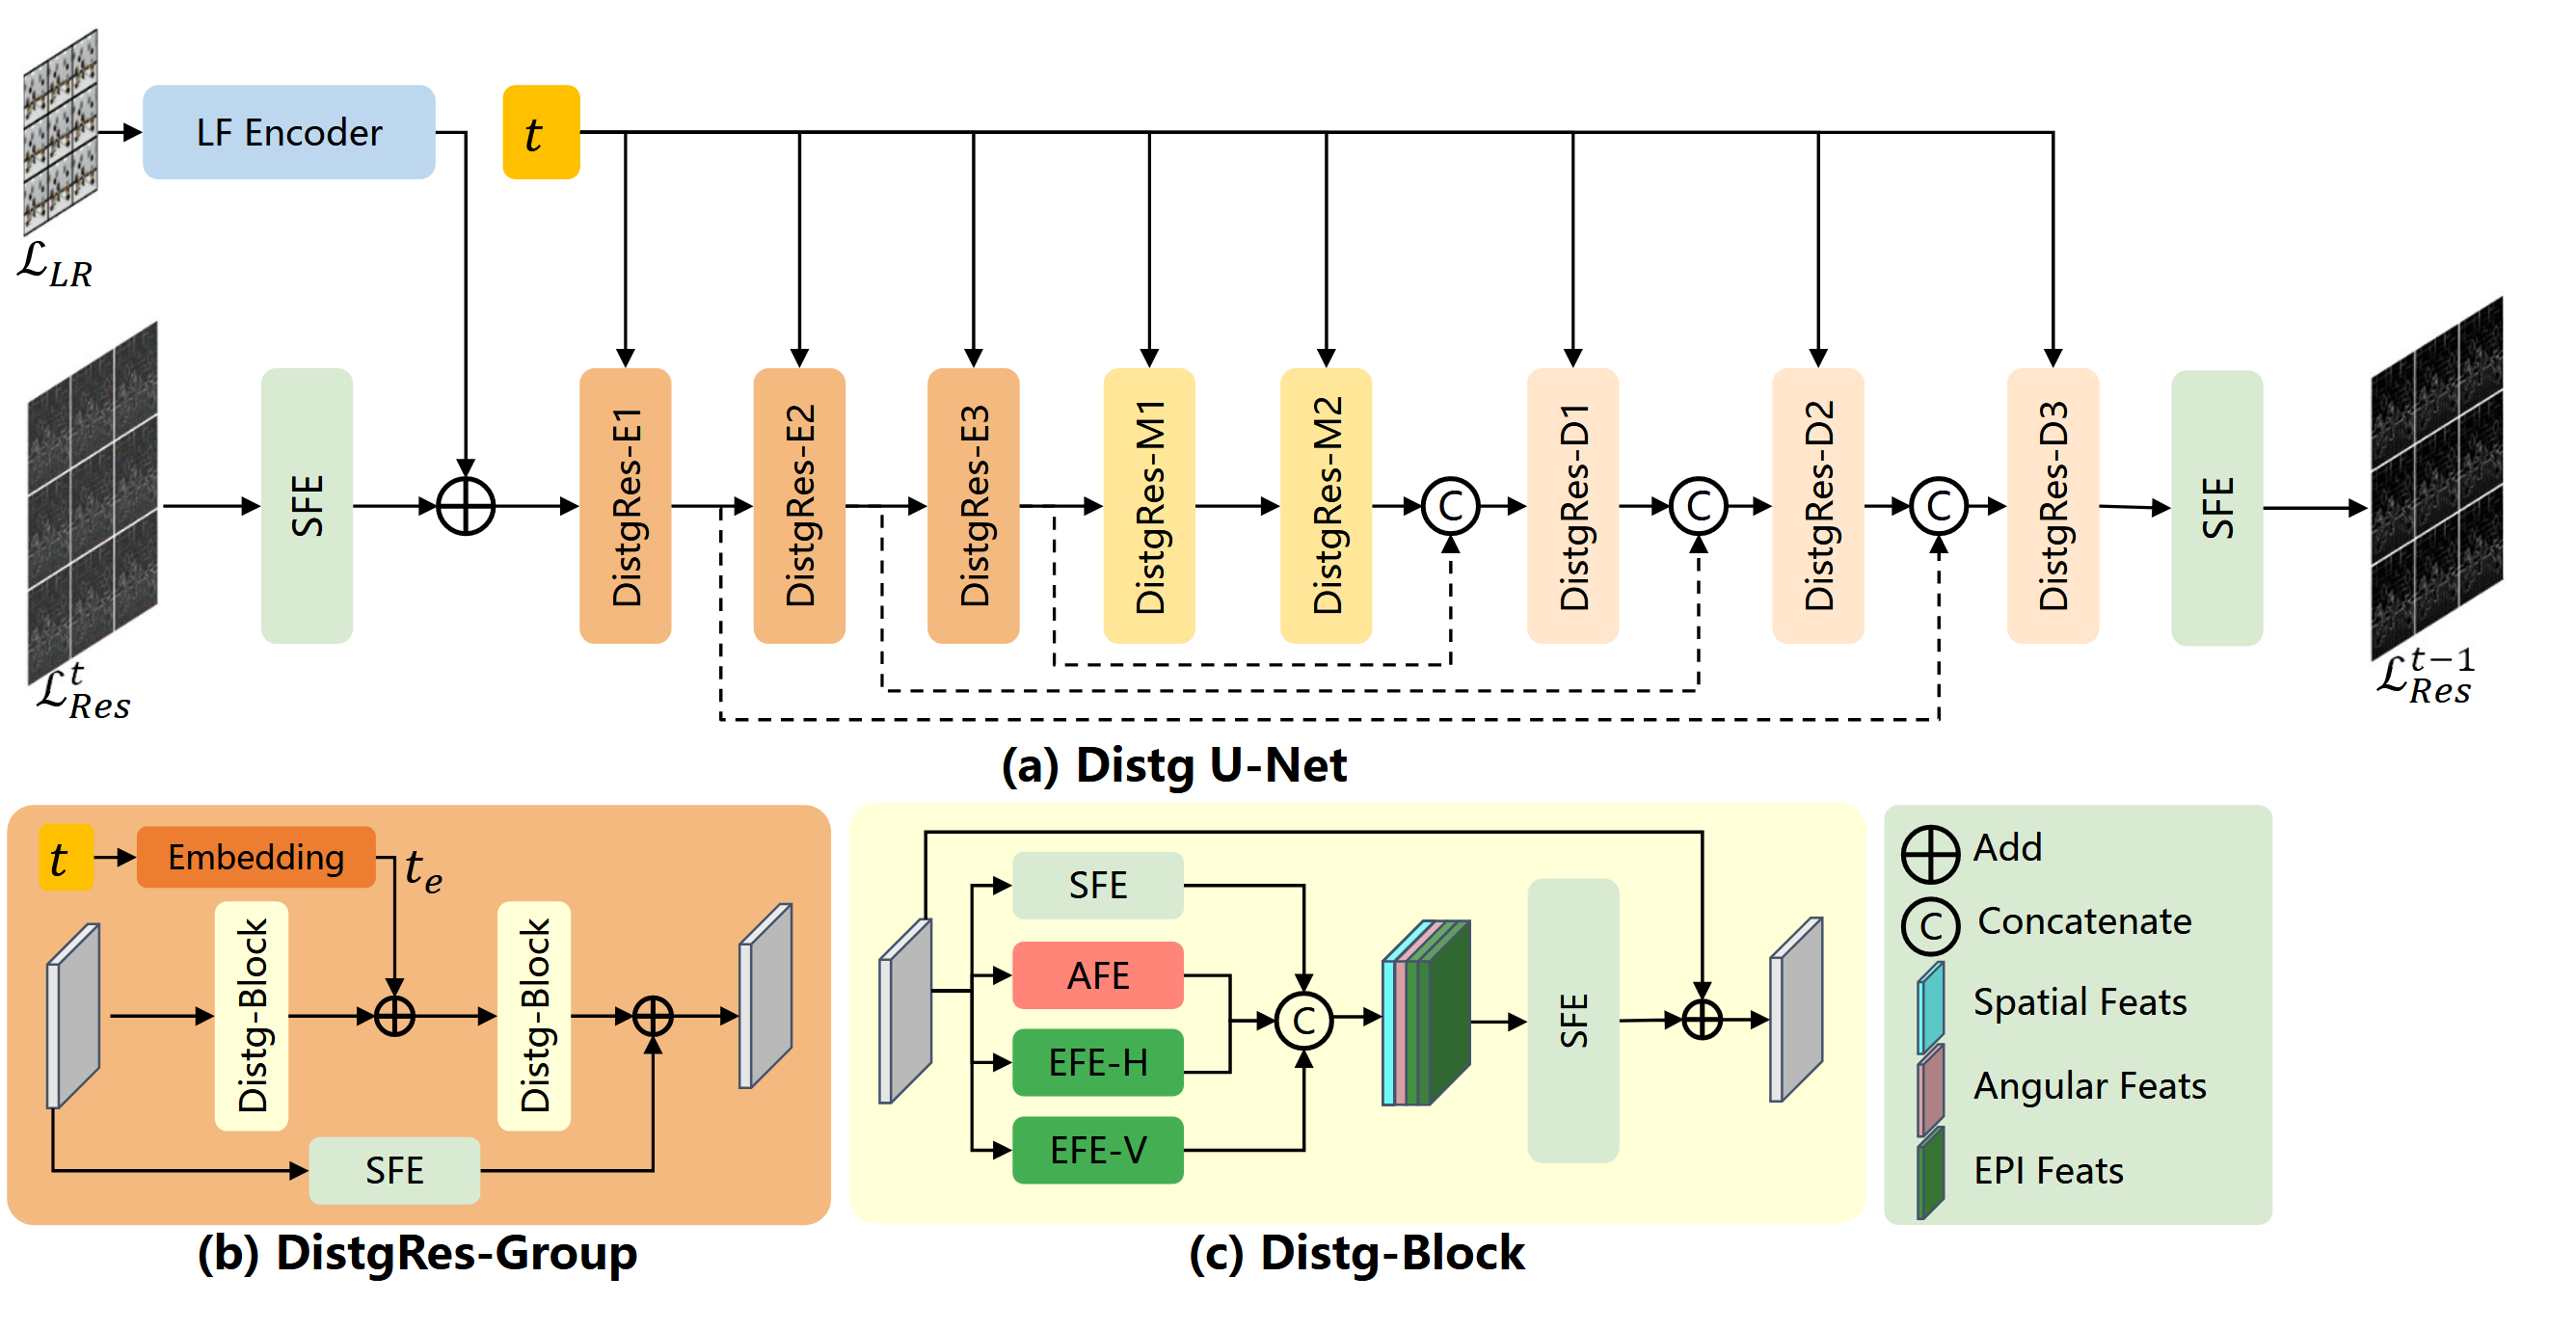
\includegraphics[width=0.9\textwidth]{models/lfsr/imgs/unet.png}
    \caption{Image taken from \cite{chaoLFSRDiffLightField2025}, visualization of the model.}
    \label{fig:distg_unet}
\end{figure}

The basic building block of the network forms the disentanglement block, shown in part (c) of figure \ref{fig:distg_unet},
it is constructed the same way as in the network described in \ref{section:distg_net} in equation \ref{eq:distgBlock}, 
but the residual connection is omitted\footnote{Despite figure \ref{fig:distg_unet} (c) displaying a residual connection, it is not used in the actual implementation.}

    $$H_{Distg}(d_{in}, d_{out}) = C_{sfe}(d_{in}, d_{out}) \circ C(144, 64, \text{kernel-size}=1) \circ P(H_{sfe}, H_{afe}, H_{efe}, H_{efe} \circ P_\sigma) ~, $$

all the modules follow the same definitions as in section \ref{section:distg_net},
apart from $C_{sfe}(d_{in}, d_{out})$.
Different from the implementation in section \ref{section:distg_net},
it might return outputs differing in channel dimension compared to its inputs

    \begin{equation*}
        C_{sfe}(d_{in}, d_{out}) = C(d_{in}, d_{out}, \text{kernel-size}=3, \text{padding}=A, \text{dilation}=A, \text{stride}=1) ~.
    \end{equation*}

The Disentaglement Residual Group builds upon the Distg Block

    $$
        H_{DistResGroup}(d_{in}, d_{out}) = s \big( H_{main}(d_{in}, d_{out}), C_{sfe}(d_{in}, d_{out}) \big) ~,
    $$

as the channel dimension of input and output might differ, 
a spatial convolution is used as a replacement for a residual connection.
The main branch of the group is made up of two cascaded disentanglement blocks,
where in between the information of the time step of the diffusion process is inferred via sinusoidal positional embeddings 

    \begin{equation} \label{eq:distg_res_main}
        H_{main}(d_{in}, d_{out}): \mathbb R^{d_{in} \times H \times W} \times \mathbb N \to \mathbb R^{d_{out} \times H \times W} ~, \\
        H_{main}(d_{in}, d_{out})(X, t) = H_{Distg}(d_{out}, d_{out}) \big( H_{Distg}(d_{in}, d_{out})(X) + \phi \circ p_{\sin}(t) \big) ~.
    \end{equation}

The mapping $\phi$ is a shallow neural network given by

    $$ \phi = F(32, 32) \circ \text{Mish} \circ F(32, 32) \circ \text{Mish} ~.$$

The addition in (\ref{eq:dist_res_main}) is to be interpreted channelwise, 
to each element of the $i$th channel of $H_{Distg}(d_{in}, d_{out})(X)$ the $i$th element of $\phi \circ p_{\sin}(t)$ is added.
The last pieces missing to describe the U-Net architecture are the upsampling and downsampling modules.
Downsampling is achieved by performing a strided convolution

    \begin{equation*}
        H_{down} = C(32, 32, \text{kernel-size}=3, \text{stride}=2, \text{padding}=1) ~.
    \end{equation*}

On the other side, upsampling is done by using a transposed convolution

    \begin{equation*}
        H_{up} = C^\top(32, 32, \text{kernel-size}=4, \text{stride}=2, \text{padding}=1) ~.
    \end{equation*}

Given initial features $F_0 \in \mathbb R^{32 \times H \times W}$,
the features in the contracting path are processed by two sequential disentanglement residual groups, 
followed by a downsampling operation

    $$ F_{i} = H_{down} \circ H_{DistResGroup}(32, 32) \circ H_{DistResGroup}(32, 32)(F_{i-1}) ~,$$

for $i = 1, 2$. The last level of the contracting path ($i = 3$) as well as the bottleneck ($i = 4, 5$) omit the downsampling

    $$ F_{i} = H_{DistResGroup}(32, 32) \circ H_{DistResGroup}(32, 32)(F_{i-1}) ~.$$

As usual for U-Net architectures, 
features from the same level are concatenated in the expanding path

    $$F_{i} = H_{up} \circ H_{DistResGroup}(32, 32) \circ H_{DistResGroup}(64, 32) \left( \big[ F_{i-1}, F_{9-i} \big] \right) ~, $$

for $i = 7, 8$. Analogously to the contracting path, the upsampling operation is omitted for the last stage of the expanding path

    $$F_{9} = H_{DistResGroup}(32, 32) \circ H_{DistResGroup}(64, 32) \left( \big[ F_{8}, F_{1} \big] \right) ~. $$
